%%%%%%%%%%%%%%%%%%%%%%%%%%%%%%%%%%%%%%%%%%%%%%%%%%%%%%%%%%%%%%%%%%%%%%
\begin{frame}[fragile]\frametitle{}
\begin{center}
{\Large Trees}
\end{center}

\end{frame}

%%%%%%%%%%%%%%%%%%%%%%%%%%%%%%%%%%%%%%%%%%%%%%%%%%%%%%%%%%%%%%%%%%%%%%
\begin{frame}
	\frametitle{Tree ADT}
	\begin{columns}[T]
		\column{0.405\textwidth}
			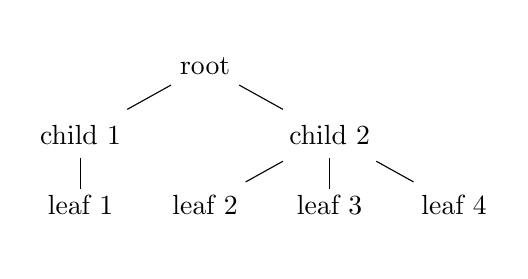
\begin{tikzpicture}[
				level distance = 2.5em,
				level 1/.style={sibling distance=9em},
				level 2/.style={sibling distance=4.5em},
				level 3/.style={sibling distance=2.25em},
			]
			\node[circle] (t1) {root} 
				child { node[circle] {child 1}
					child { node[circle] {leaf 1}}
				}
				child { node[circle] {child 2}
					child { node[circle] {leaf 2}}
					child { node[circle] {leaf 3}}
					child { node[circle] {leaf 4}}
				};
			\end{tikzpicture}
		\column{0.555\textwidth}
		\begin{itemize}
			\item The \textit{root node} is the node that has no \textit{parent}.
				
			\item A node can have \textit{children}.
				
			\item A node without children is called a \textit{leaf}.
				
			\item Two nodes with the same \textit{parent} are \textit{siblings}.
				
			\item \textit{Descendants} are found by repeatedly following child-relations.
				
			\item \textit{Ancestors} are found by repeatedly following parent-relations.
		\end{itemize}
	\end{columns}
\end{frame}

%%%%%%%%%%%%%%%%%%%%%%%%%%%%%%%%%%%%%%%%%%%%%%%%%%%%%%%%%%%%%%%%%%%%%%
\begin{frame}
	\frametitle{Quick check}
	
	\begin{columns}[T]
		\column{0.405\textwidth}
			\begin{tikzpicture}[
				level distance = 2.5em,
				level 1/.style={sibling distance=2em},
				level 2/.style={sibling distance=4.5em},
				level 3/.style={sibling distance=2.25em},
			]
			\node[circle] (t1) {r}
				child { node[circle] {k}
					child { node[circle] {d}}
				}
				child { node[circle] {a} }
				child { node[circle] {b} }
				child { node[circle] {e} 
					child { node[circle] {g} }
					child { node[circle] {h}
						child { node[circle] {i}}
					}
				}
				child { node[circle] {f} };
			\end{tikzpicture}
		\column{0.555\textwidth}
		
			\begin{itemize}
				\item Let $c(v)$ be the set of children of $v$.
				\item Let $d(v)$ be the set of descendants of $v$.
				\item Let $s(v)$ be the set of siblings of $v$.
				\item Let $a(v)$ be the set of ancestors of $v$.
				\item Let $p(v)$ be the parent of $v$.
				\item What is: $|c(k)| + |d(p(g))| + \sum\limits_{v \in a(h)} |s(v)|$?
				\begin{itemize}
					\item 4
					\item 8
					\item 12
					\item I don't know
				\end{itemize}
			\end{itemize}
	\end{columns}
	
Arithmetic time:
		$c(k) = \{d\}$, $p(g) = e$, $d(e) = \{g,h,i\}$, $a(h) = \{r,e\}$, $s(r) = \emptyset$, $s(e) = \{k,a,b,f\}$. So the
		final answer is: $1+3+4=8$.
\end{frame}


%%%%%%%%%%%%%%%%%%%%%%%%%%%%%%%%%%%%%%%%%%%%%%%%%%%%%%%%%%%%%%%%%%%%%%
\begin{frame}
	\frametitle{Depth of a node}

	\begin{columns}[T]
		\column{0.405\textwidth}
			\begin{tikzpicture}[
				level distance = 2.5em,
				level 1/.style={sibling distance=9em},
				level 2/.style={sibling distance=4.5em},
				level 3/.style={sibling distance=2.25em},
			]
			\node[circle] (t1) {root}
				child { node[circle]   {child 1}
					child { node[circle] {l1}}
				}
				child { node[circle]   {child 2}
					child { node[circle] {l2}}
					child { node[circle] {l3}}
					child { node[circle] {l4}}
				};
			\end{tikzpicture}
		\column{0.555\textwidth}
		\begin{itemize}
			\item The \textit{depth} of a \alert<5->{node} is the distance to the root.
				
			\item So depth(root) = 0.
			\item And depth(l2) = 2.
				
			\item The \textit{height} of a \alert<5->{tree} is the length of the longest path from root to leaf.
				
			\item So the height of this tree is 3.
				
			\item Note: Every book/author has their own definition of these things! Including our book :(
		\end{itemize}
	\end{columns}
	
\end{frame}

%%%%%%%%%%%%%%%%%%%%%%%%%%%%%%%%%%%%%%%%%%%%%%%%%%%%%%%%%%%%%%%%%%%%%%

\begin{frame}
	\frametitle{Depth of a node}

	\begin{columns}[T]
		\column{0.405\textwidth}
			\begin{tikzpicture}[
				level distance = 2.5em,
				level 1/.style={sibling distance=9em},
				level 2/.style={sibling distance=4.5em},
				level 3/.style={sibling distance=2.25em},
			]
			\node[circle] (t1) {root}
				child { node[circle]   {child 1}
					child { node[circle] {l1}}
				}
				child { node[circle]   {child 2}
					child { node[circle] {l2}}
					child { node[circle] {l3}}
					child { node[circle] {l4}}
				};
			\end{tikzpicture}
		\column{0.555\textwidth}
		Alternative definition for height: How can we also describe the tree height of a tree $T$?
			
			\begin{itemize}
				\item $\max\limits_{v\in T}({\textit{depth}(v)})-1$
				\item $\max\limits_{v\in T}({\textit{depth}(v)})$
				\item $\max\limits_{v\in T}({\textit{depth}(v)})+1$
			\end{itemize}
	\end{columns}
	
	A tree of height one:
	
			\begin{itemize}
				\item Remember that a tree of height one is just the root, which is at depth $0$. So it cannot be A or B.
				\item Then remember that depth is the distance, but height is the length of the path. These differ by 1, so C is the right answer.
			\end{itemize}
				
\end{frame}

%%%%%%%%%%%%%%%%%%%%%%%%%%%%%%%%%%%%%%%%%%%%%%%%%%%%%%%%%%%%%%%%%%%%%%

\begin{frame}
	\frametitle{An implementation}
	
		\begin{itemize}
				\item How can we implement such a tree structure?
				\item By using nodes that are \textit{linked} together to form a tree!
	\end{itemize}
	
	\begin{columns}[t]
		\column{0.535\textwidth}
	\lstinputlisting{src/tree.py}
			
		\column{0.505\textwidth}
	\lstinputlisting{src/treenode.py}
			
	\end{columns}
\end{frame}

%%%%%%%%%%%%%%%%%%%%%%%%%%%%%%%%%%%%%%%%%%%%%%%%%%%%%%%%%%%%%%%%%%%%%%
\begin{frame}
	\frametitle{Node Depth}

			Find the depth of a node is easy if we know the depth of the parent.
		
		\lstinputlisting{src/nodedepth.py}
\end{frame}

%%%%%%%%%%%%%%%%%%%%%%%%%%%%%%%%%%%%%%%%%%%%%%%%%%%%%%%%%%%%%%%%%%%%%%

\begin{frame}
	\frametitle{Tree Height}

			The height of the tree is the max depth + 1! 	
		
		\lstinputlisting{src/treeheight.py}
\end{frame}

%%%%%%%%%%%%%%%%%%%%%%%%%%%%%%%%%%%%%%%%%%%%%%%%%%%%%%%%%%%%%%%%%%%%%%
\begin{frame}
	\frametitle{Getting all the leaves}
How can we get all the leaves from a tree?
		
		\lstinputlisting{src/treeleaves.py}
\end{frame}

%%%%%%%%%%%%%%%%%%%%%%%%%%%%%%%%%%%%%%%%%%%%%%%%%%%%%%%%%%%%%%%%%%%%%%

\begin{frame}
	\frametitle{The Tree ADT}
		\begin{itemize}
				\item Different implementations of trees, give you different ADTs.
				\item The book uses one which is \textit{position}-focused.
				\item The properties are always the same, just the functions and how to call them can be different.
		\end{itemize}	
\end{frame}

%%%%%%%%%%%%%%%%%%%%%%%%%%%%%%%%%%%%%%%%%%%%%%%%%%%%%%%%%%%%%%%%%%%%%%
\begin{frame}
	\frametitle{Alternative implementation}
			Every node in a tree, is the root to a subtree!
		
		\begin{columns}[T]
			\column{0.455\textwidth}
				
			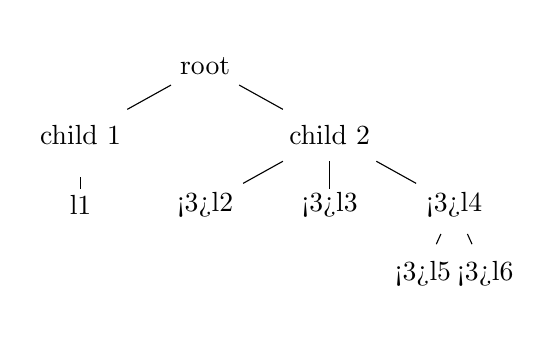
\begin{tikzpicture}[
				level distance = 2.5em,
				level 1/.style={sibling distance=9em},
				level 2/.style={sibling distance=4.5em},
				level 3/.style={sibling distance=2.25em},
			]
			\node[circle] (t1) {root}
				child { node[circle]   {child 1}
					child { node[circle] {l1}}
				}
				child { node[circle]   {child 2} % ,
					child { node[circle] {\alert<3>{l2}}}
					child { node[circle] {\alert<3>{l3}}}
					child { node[circle] {\alert<3>{l4}}
						child { node[circle] {\alert<3>{l5}}}
						child { node[circle] {\alert<3>{l6}}}
					}
				};
			\end{tikzpicture}
			
			\column{0.455\textwidth}

					In the example on the right, child 2 is the root of the subtree drawn in red.
		\end{columns}
\end{frame}

%%%%%%%%%%%%%%%%%%%%%%%%%%%%%%%%%%%%%%%%%%%%%%%%%%%%%%%%%%%%%%%%%%%%%%

\begin{frame}
	\frametitle{Alternative implementation}
By implementing it like this, we have no need for \texttt{TreeNode}s. All nodes are just \texttt{Tree}s!

		\lstinputlisting{src/tree_alt.py}
\end{frame}

%%%%%%%%%%%%%%%%%%%%%%%%%%%%%%%%%%%%%%%%%%%%%%%%%%%%%%%%%%%%%%%%%%%%%%
\begin{frame}
	\frametitle{Alternative implementation: Tree Height}
How do we determine the height in this set-up?
	
	\lstinputlisting{src/tree_alt_height.py}
\end{frame}

%%%%%%%%%%%%%%%%%%%%%%%%%%%%%%%%%%%%%%%%%%%%%%%%%%%%%%%%%%%%%%%%%%%%%%
\begin{frame}
	\frametitle{Why have one implementation over the other?}

				\begin{itemize}
				\item Which implementation should you use?
					\item	It depends of course ;)
						\item What information do you need to store for your use case?
	\end{itemize}
	
\end{frame}

% %%%%%%%%%%%%%%%%%%%%%%%%%%%%%%%%%%%%%%%%%%%%%%%%%%%%%%%%%%%%%%%%%%%%%%
% \begin{frame}
	% \frametitle{Binary Trees}
	% \begin{center}
			% \begin{tikzpicture}[level/.style={sibling distance = 3cm, %->,>=stealth',
		  % level distance = 1cm},
			  % treenode/.style = {align=center, inner sep=0pt, text centered,
		    % font=\sffamily},
		  % arn_n/.style = {treenode, circle, white, font=\sffamily\bfseries, draw=black,
		    % fill=black, text width=1.5em},% arbre rouge noir, noeud noir
		  % arn_r/.style = {treenode, circle, red, draw=red,
		    % text width=1.5em, very thick},% arbre rouge noir, noeud rouge
		  % arn_x/.style = {treenode, rectangle, draw=black,
		    % minimum width=0.5em, minimum height=0.5em}% arbre rouge noir, nil
			% ]
			% \node [arn_n] {33}
    % child{ node [arn_r] {15}
            % child{ node [arn_n] {10}
            	% % child{ node [arn_r] {5} edge from parent node[above left]{$x$}}
							% % child{ node [arn_x] {}}
            % }
            % child{ node [arn_n] {20}
							% % child{ node [arn_r] {18}}
							% % child{ node [arn_x] {}}
            % }
    % }
    % child{ node [arn_r] {47}
            % child{ node [arn_n] {38}
							% % child{ node [arn_r] {36}}
							% % child{ node [arn_r] {39}}
            % }
            % child{ node [arn_n] {51}
							% % child{ node [arn_r] {49}}
							% % child{ node [arn_x] {}}
            % }
		% }
% ;
% \end{tikzpicture}
	% \end{center}
	
	% {\scriptsize Tikz taken from: \url{http://texample.net/tikz/examples/red-black-tree/}}

% \end{frame}

%%%%%%%%%%%%%%%%%%%%%%%%%%%%%%%%%%%%%%%%%%%%%%%%%%%%%%%%%%%%%%%%%%%%%%
\begin{frame}
	\frametitle{Binary Trees}

			\begin{itemize}
				\item Every node has at most 2 children.
					
				\item One \textit{left} child and one \textit{right} child.
			\end{itemize}
		
		A binary tree is \textit{proper} or \textit{full} if all nodes have either 0 or 2 children.

		
		\begin{columns}[T]
			\column{0.455\textwidth}
				
			\begin{tikzpicture}[
				level distance = 2.5em,
				level 1/.style={sibling distance=9em},
				level 2/.style={sibling distance=4.5em},
				level 3/.style={sibling distance=2.25em},
			]
			\node[circle] (t1) {root}
				child { node[circle]   {child 1}
					child { node[circle] {l1}}
					child { node[circle] {l2}}
				}
				child { node[circle]   {child 2}
					child { node[circle] {l3}}
					child { node[circle] {l4}
						child { node[circle] {l5}}
						child { node[circle] {l6}}
					}
				};
			\end{tikzpicture}
			\column{0.455\textwidth}
				
				Is this tree full?
				\begin{enumerate}[A.]
					\item Yes
					\item No
					\item I don't know
				\end{enumerate}
		\end{columns}
\end{frame}

%%%%%%%%%%%%%%%%%%%%%%%%%%%%%%%%%%%%%%%%%%%%%%%%%%%%%%%%%%%%%%%%%%%%%%

% \begin{frame}
	% \frametitle{Tree properties pt2}
	% \begin{center}
		% 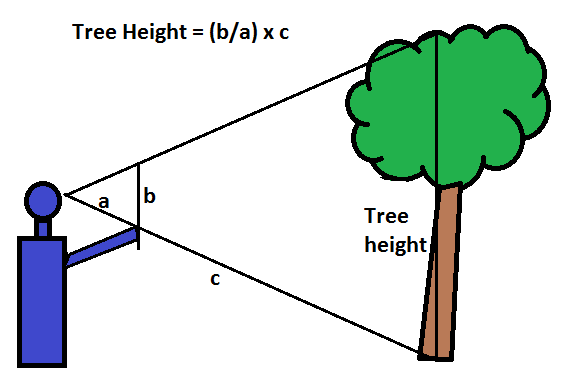
\includegraphics[width=0.6\textwidth]{images/stick.png}\\
		% \hspace*{15pt}\hbox{\scriptsize Image By:\thinspace{\itshape Edfrank01}}
		% % https://commons.wikimedia.org/wiki/File:Stick_measurement.png
	% \end{center}
% \end{frame}

% \begin{frame}
	% \frametitle{Tree time}
	% \begin{center}
		% 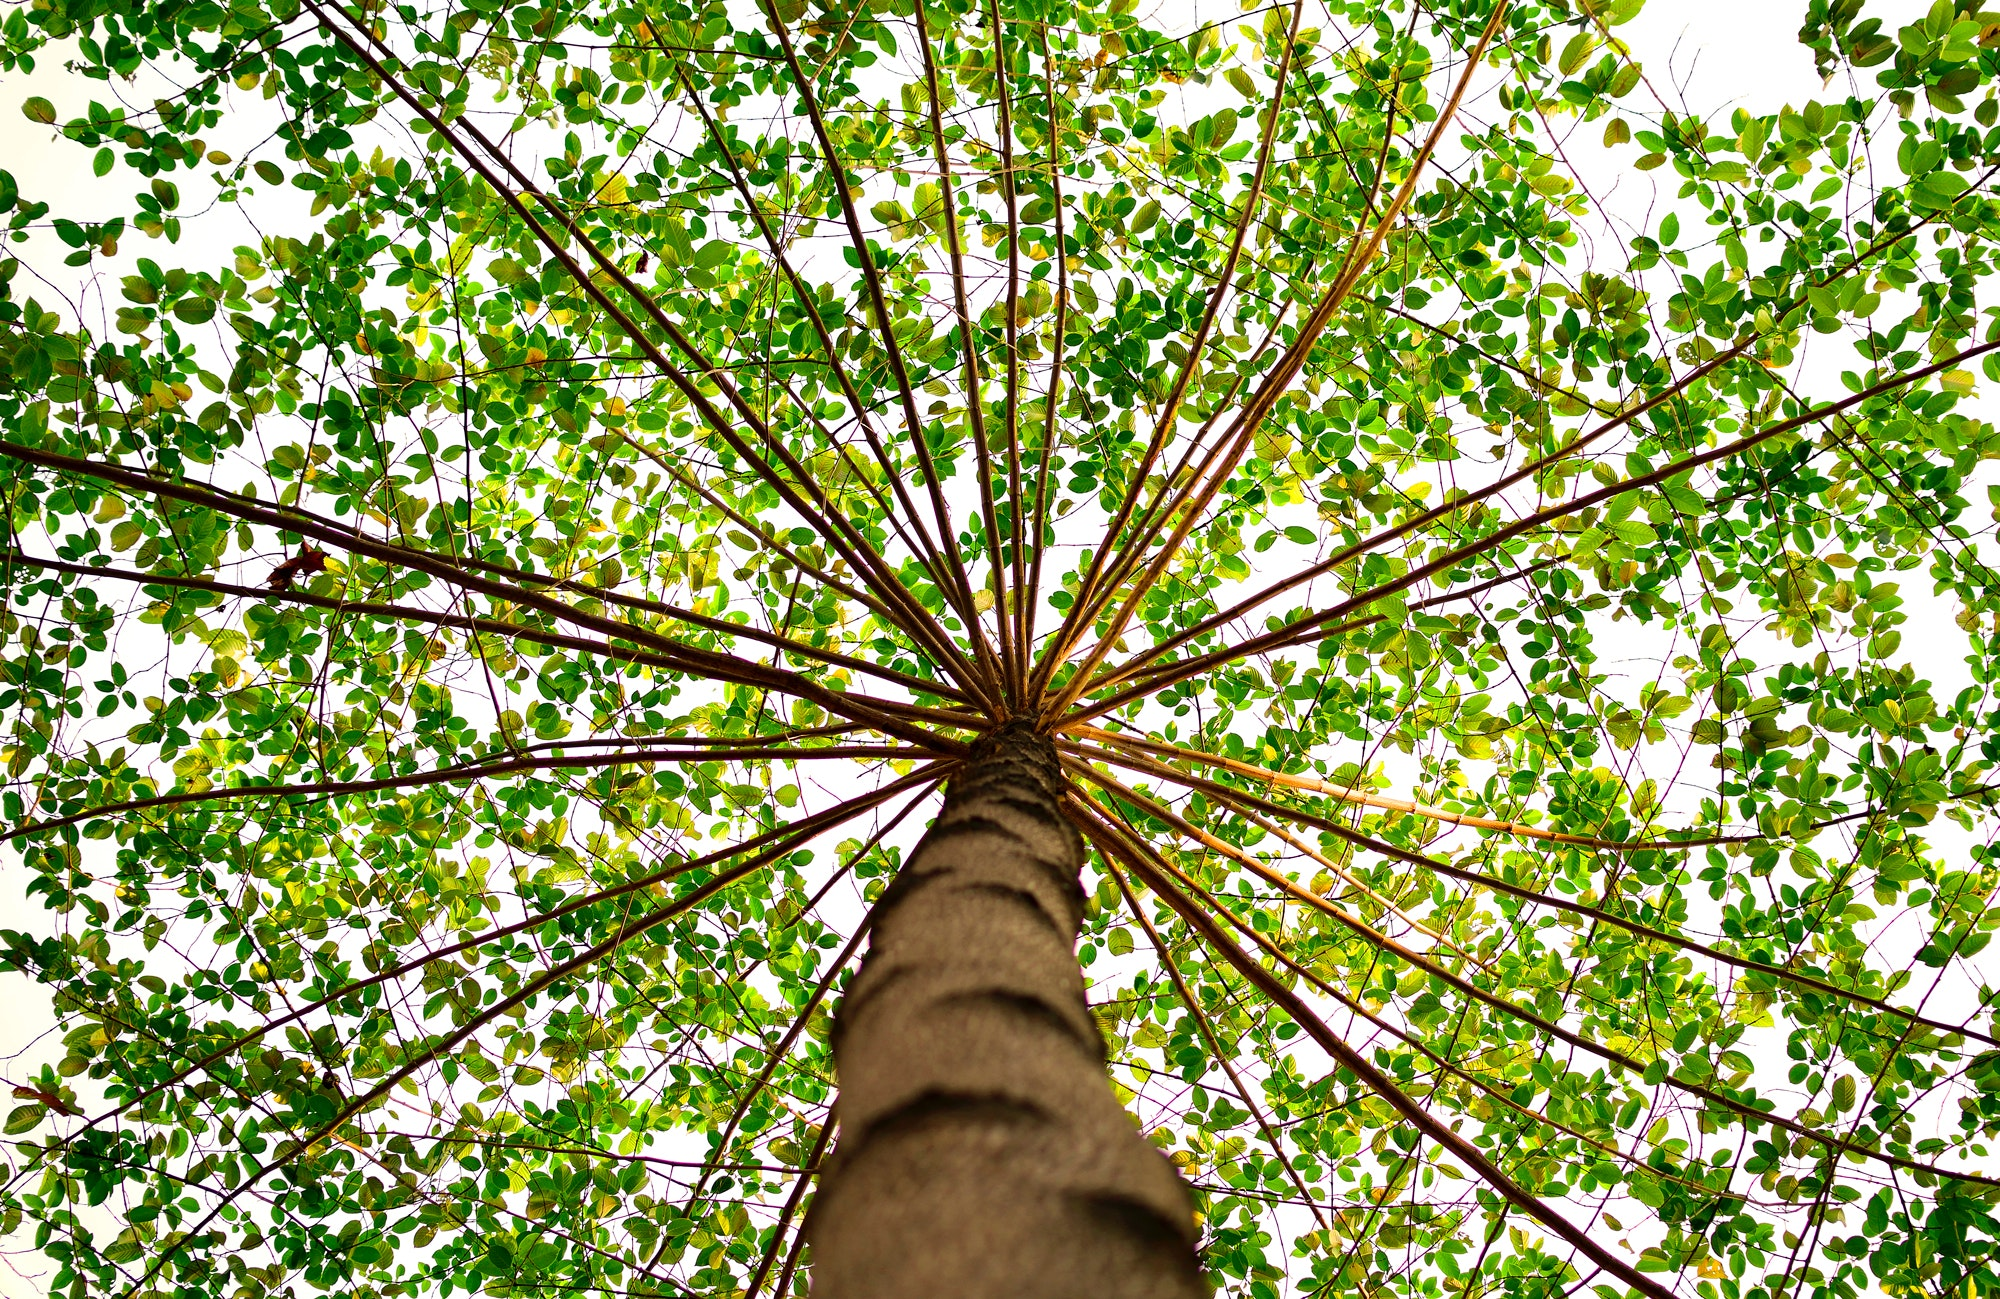
\includegraphics[width=0.6\textwidth]{images/tree.jpg}\\
		% \hspace*{15pt}\hbox{\scriptsize Image By:\thinspace{\itshape George achik}}
		% % https://commons.wikimedia.org/wiki/File:Last_summer_time_tree_and_evening_time,_In_Srimongol,_Bangladesh.jpg
	% \end{center}
% \end{frame}


% \begin{frame}
	% \frametitle{Tree traversals}
	% \framesubtitle{Walking through our tree}

	% \begin{center}
		% 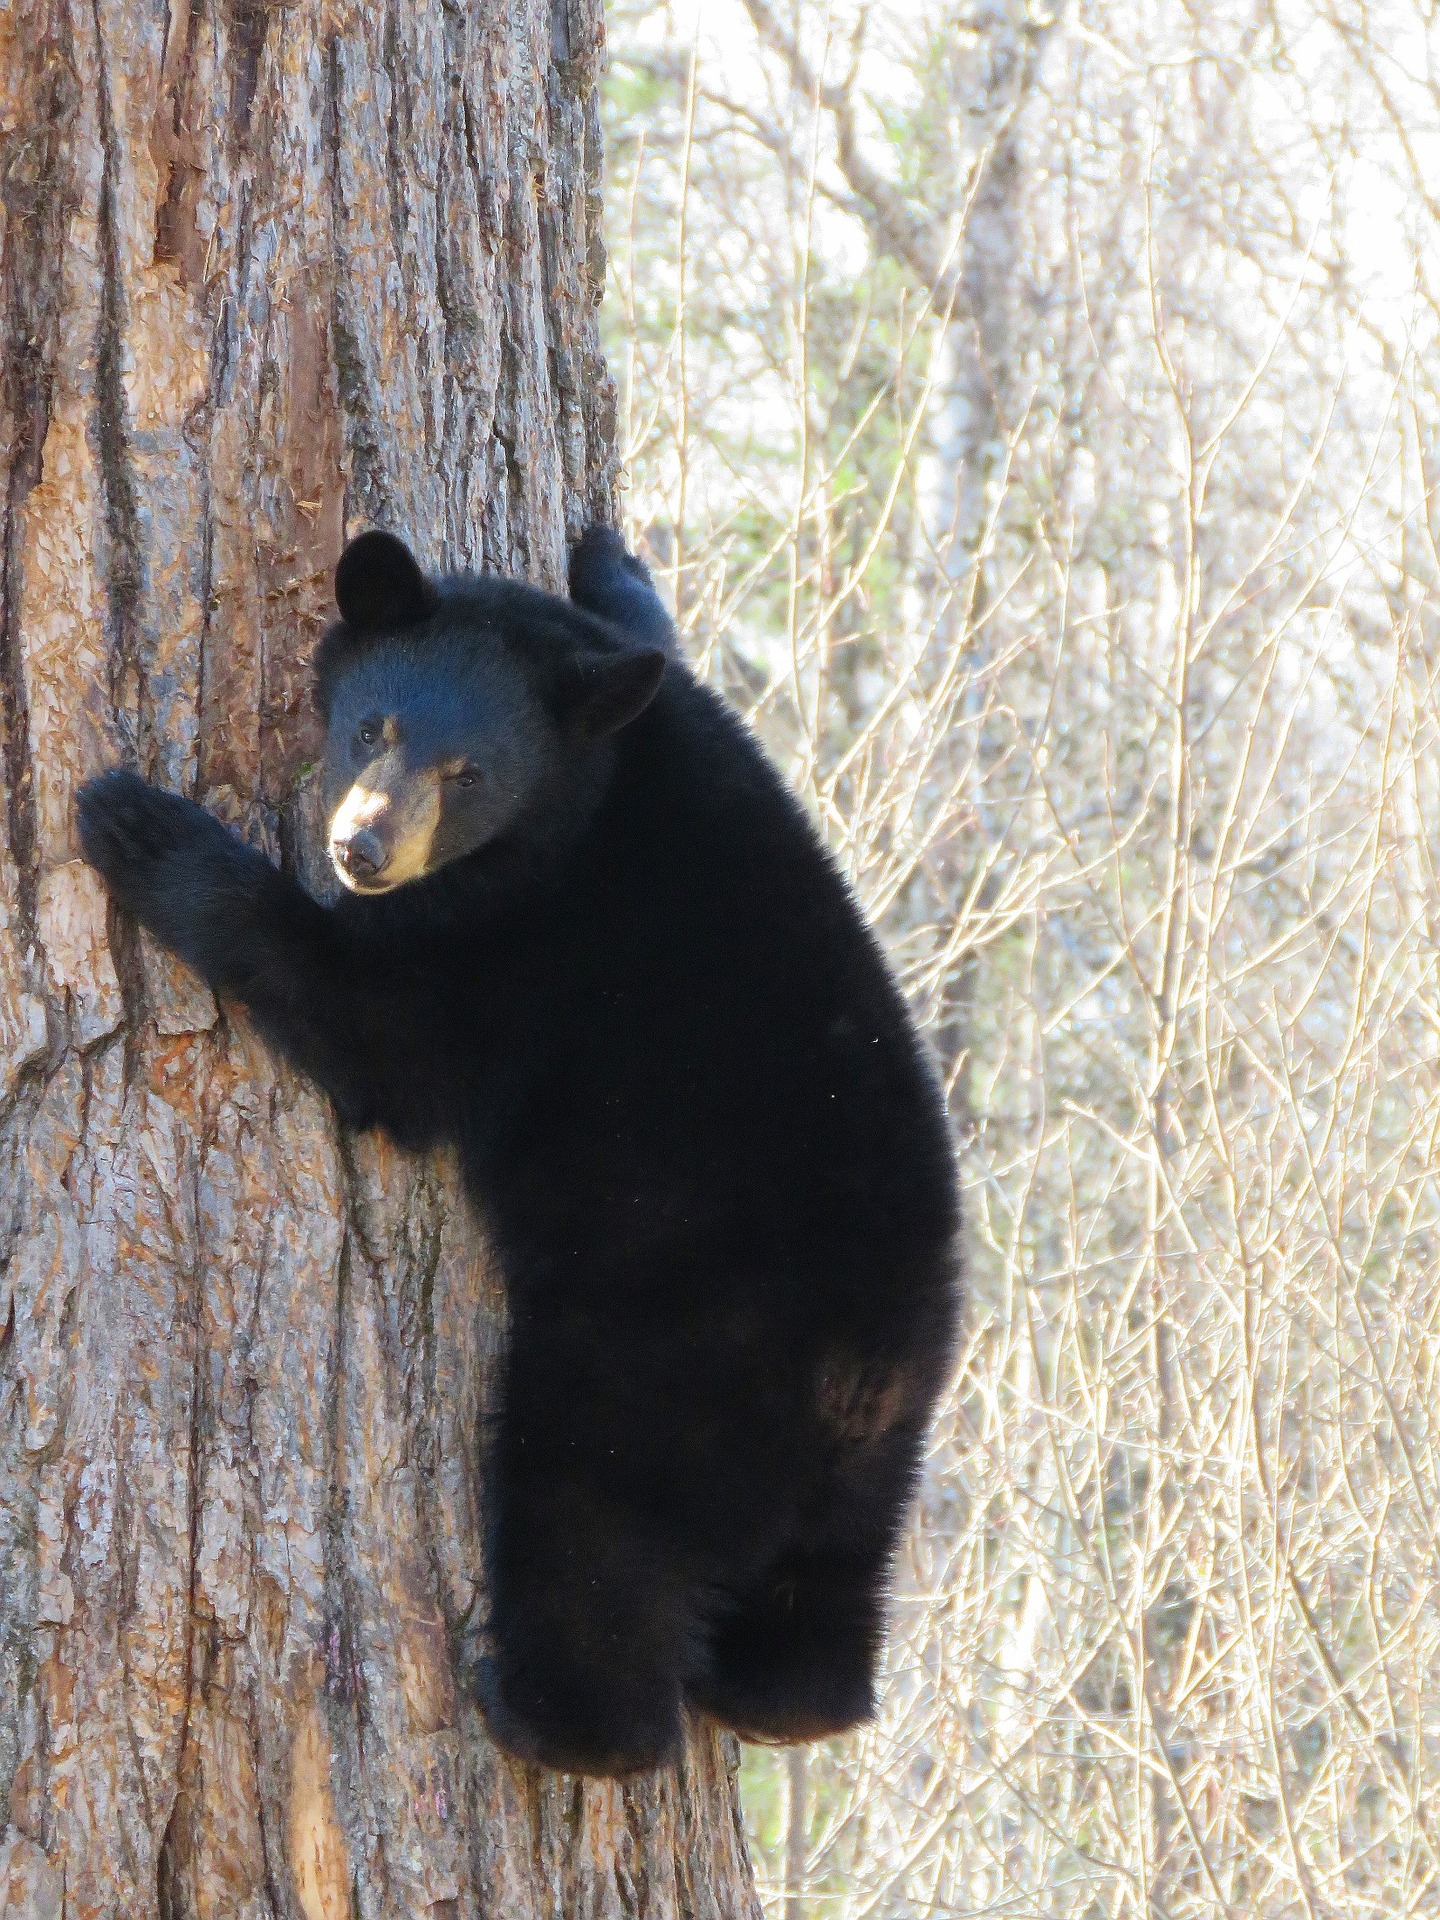
\includegraphics[trim={0 4cm 0 4cm},clip, width=0.65\textwidth]{images/bearcub.jpg}\\
		% \hspace*{15pt}\hbox{\scriptsize Image By:\thinspace{\itshape Skeeze}}
		% % https://pixabay.com/photos/bear-cub-brown-climbing-tree-1576559/
	% \end{center}

% \end{frame}

%%%%%%%%%%%%%%%%%%%%%%%%%%%%%%%%%%%%%%%%%%%%%%%%%%%%%%%%%%%%%%%%%%%%%%
\begin{frame}
	\frametitle{Iterating over the nodes}
	
		Finding all the nodes: If you want to iterate over the tree, you can do so in many different orders. Three common ones for binary trees are:
			\begin{itemize}
				\item Pre-order traversal
				\item In-order traversal
				\item Post-order traversal
			\end{itemize}
\end{frame}

%%%%%%%%%%%%%%%%%%%%%%%%%%%%%%%%%%%%%%%%%%%%%%%%%%%%%%%%%%%%%%%%%%%%%%
\begin{frame}
	\frametitle{Pre-order traversal}
			\begin{columns}[T]
				\column{0.455\textwidth}
				\begin{itemize}
					\item First give the value of the current node.
					\item Then a pre-order traversal of the left child.
					\item Then a pre-order traversal of the right child.
				\end{itemize}
				\column{0.455\textwidth}
				
					\begin{tikzpicture}[
						level distance = 2.5em,
						level 1/.style={sibling distance=9em},
						level 2/.style={sibling distance=4.5em},
						level 3/.style={sibling distance=2.25em},
					]
					\node[circle] (t1) {\alert<3>{1}}
					child { node[circle]   {\alert<4>{2}}
						child { node[circle] {\alert<5>{3}}}
						}
						child { node[circle]   {\alert<6>{4}}
							child { node[circle] {\alert<7>{5}}}
							child { node[circle] {\alert<8>{6}}
								child { node[circle] {\alert<9>{7}}}
								child { node[circle] {\alert<10>{8}}}
							}
						};
					\end{tikzpicture}
			\end{columns}

Amsterdam, Rotterdam, no not that kind of topology!:
				\begin{itemize}
					\item Gives us a \textit{topological} order of the tree.
					\item If all nodes represent jobs, and job $i$ depends on it's parent job $p$ then this gives us an order in which we can	do all jobs, satisfying these dependencies.
			\end{itemize}
\end{frame}

%%%%%%%%%%%%%%%%%%%%%%%%%%%%%%%%%%%%%%%%%%%%%%%%%%%%%%%%%%%%%%%%%%%%%%
\begin{frame}
	\frametitle{In-order traversal}
			\begin{columns}[T]
				\column{0.455\textwidth}
				\begin{itemize}
					\item First an in-order traversal of the left child.
					\item Then give the value of the current node.
					\item Then an in-order traversal of the right child.
				\end{itemize}
				\column{0.455\textwidth}
					\begin{tikzpicture}[
						level distance = 2.5em,
						level 1/.style={sibling distance=9em},
						level 2/.style={sibling distance=4.5em},
						level 3/.style={sibling distance=2.25em},
					]
					\node[circle] (t1) {1}
					child { node[circle]   {2}
						child { node[circle] {3}}
						}
						child { node[circle]   {4}
							child { node[circle] {5}}
							child { node[circle] {6}
								child { node[circle] {7}}
								child { node[circle] {8}}
							}
						};
					\end{tikzpicture}
			\end{columns}
				What is the order of nodes now?
					\begin{itemize}
						\item 1,2,3,4,5,6,7,8
						\item 3,2,1,5,4,7,6,8
						\item 3,2,8,7,6,5,4,1
						\item 8,7,6,5,4,3,2,1
					\end{itemize}
		
\end{frame}

%%%%%%%%%%%%%%%%%%%%%%%%%%%%%%%%%%%%%%%%%%%%%%%%%%%%%%%%%%%%%%%%%%%%%%
\begin{frame}
	\frametitle{Post-order traversal}
			\begin{columns}[T]
				\column{0.455\textwidth}
				\begin{itemize}
					\item First a post-order traversal of the left child.
					\item Then a post-order traversal of the right child.
					\item Then give the value of the current node.
				\end{itemize}
				\column{0.455\textwidth}
					\begin{tikzpicture}[
						level distance = 2.5em,
						level 1/.style={sibling distance=9em},
						level 2/.style={sibling distance=4.5em},
						level 3/.style={sibling distance=2.25em},
					]
					\node[circle] (t1) {\alert<10>{1}}
					child { node[circle]   {\alert<4>{2}}
						child { node[circle] {\alert<3>{3}}}
						}
						child { node[circle]   {\alert<9>{4}}
							child { node[circle] {\alert<5>{5}}}
							child { node[circle] {\alert<8>{6}}
								child { node[circle] {\alert<6>{7}}}
								child { node[circle] {\alert<7>{8}}}
							}
						};
					\end{tikzpicture}
			\end{columns}
				What is the order of nodes now?
					\begin{itemize}
						\item 1,2,3,4,5,6,7,8
						\item 3,2,5,8,7,6,4,1
						\item 3,2,8,7,6,5,4,1
						\item 8,7,6,5,4,3,2,1
					\end{itemize}

				Used to delete a tree (first delete your children, before deleting yourself).

\end{frame}

%%%%%%%%%%%%%%%%%%%%%%%%%%%%%%%%%%%%%%%%%%%%%%%%%%%%%%%%%%%%%%%%%%%%%%
\begin{frame}
	\frametitle{Limiting the height}
		If we can somehow limit the height to be $\Theta(\log n)$ we are all set.
	
	This is where the tens of options come in...
	\begin{itemize}
		\item AVL-trees
		\item Red-Black trees
		\item Splay-trees
		\item And many more\dots
	\end{itemize}
\end{frame}

%%%%%%%%%%%%%%%%%%%%%%%%%%%%%%%%%%%%%%%%%%%%%%%%%%%%%%%%%%%%%%%%%%%%%%
\begin{frame}
	\frametitle{AVL-Trees}
	\framesubtitle{Named after Adel'son-Vel'skii and Landis}

AVL-trees:It is a binary search tree, with one more constraint:
			The height of the left-subtree and right-subtree of a node differ by at most 1 for all nodes in the tree.

	\begin{columns}[T]
		\column{0.455\textwidth}

		\begin{tikzpicture}[
			level distance = 2.5em,
			level 1/.style={sibling distance=9em},
			level 2/.style={sibling distance=4.5em},
			level 3/.style={sibling distance=2.25em},
			]
			\node[circle] (t1) {12}
			child { node[circle]   {3}
				child[draw=white] { }
				child { node[circle] {9}}
			}
			child { node[circle]   {25}
				child { node[circle] {14}}
				child { node[circle] {29}
					child { node[circle] {26}}
					child { node[circle] {32}}
				}
			};
		\end{tikzpicture}
		\column{0.455\textwidth}

			Is this tree an AVL-tree?
		
			Yes :)	
	\end{columns}
\end{frame}

%%%%%%%%%%%%%%%%%%%%%%%%%%%%%%%%%%%%%%%%%%%%%%%%%%%%%%%%%%%%%%%%%%%%%%
\begin{frame}
	\frametitle{AVL-trees}
		\begin{itemize}
			\item This guarantees the height to be $\Theta(\log n)$ (check the book for a proof if you want).
			\item How do we now insert or delete nodes from this AVL tree?
	\end{itemize}
\end{frame}

%%%%%%%%%%%%%%%%%%%%%%%%%%%%%%%%%%%%%%%%%%%%%%%%%%%%%%%%%%%%%%%%%%%%%%
\begin{frame}
	\frametitle{Inserting items}

Observations:
		\begin{itemize}
			\item If we insert like we did in a ``regular'' binary search tree\dots
			\item Then we only upset (potentially) the ancestors of the node where we insert it.
				
			\item Let's look at an example ;)
		\end{itemize}
	
Inserting an item:
		\begin{columns}[T]
			\column{0.455\textwidth}

			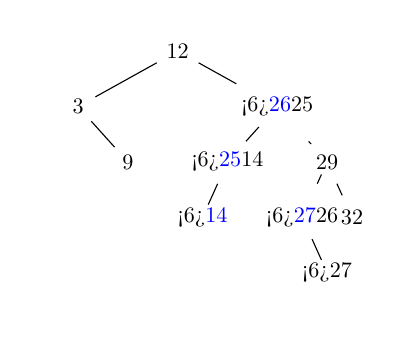
\begin{tikzpicture}[
				level distance = 2.5em,
				level 1/.style={sibling distance=9em},
				level 2/.style={sibling distance=4.5em},
				level 3/.style={sibling distance=2.25em},
				scale=0.8,transform shape
				]
				\node[circle] (t1) {12}
				child { node[circle]   {3}
					child[draw=white] { }
					child { node[circle] {9}}
				}
				child { node[circle]   {\alt<6>{\color{blue}26}{25}}
					child { node[circle] {\alt<6>{\color{blue}{25}}{14}}
						child[] { node[circle] {\alt<6>{\color{blue}{14}}{}}}
						child[draw=white] { }
					}
					child { node[circle] {29}
						child { node[circle] {\alt<6>{\color{blue}27}{26}}
							child[draw=white] { }
							child[] { node[circle] {\alt<6>{}{27}}}
						}
						child { node[circle] {32}}
					}
				};
			\end{tikzpicture}
			\column{0.455\textwidth}
			\begin{itemize}
				\item Two items are now upsetting the AVL-property.
					
				\item So we need to fix that!
					
				\item We can do so by \textit{rotating} some nodes around.
					
				\item To end up with this.
			\end{itemize}
		\end{columns}
\end{frame}

%%%%%%%%%%%%%%%%%%%%%%%%%%%%%%%%%%%%%%%%%%%%%%%%%%%%%%%%%%%%%%%%%%%%%%
\begin{frame}
	\frametitle{A tri-node restructering}
	\begin{columns}[T]
		\column{0.455\textwidth}
			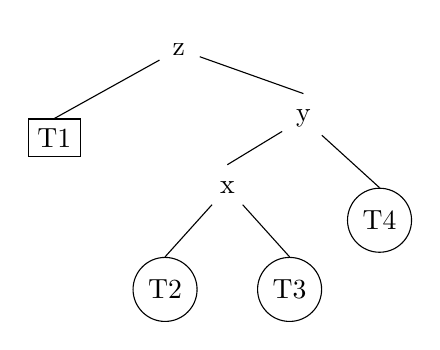
\begin{tikzpicture}[
				level distance = 2.5em,
				level 1/.style={sibling distance=9em},
				level 2/.style={sibling distance=5.5em},
				level 3/.style={sibling distance=4.5em},
				child anchor =north
				]
				\node[circle] (t1) {z}
				child { node[draw=black, anchor = north]   {T1}
				}
				child { node[circle]   {y}
					child { node[circle] {x}
						child { node[circle, anchor = north, draw=black] {T2}}
						child { node[circle, anchor = north, draw=black] {T3}}
					}
					child { node[circle, anchor = north, draw=black] {T4}
					}
				};
			\end{tikzpicture}
		\column{0.455\textwidth}
		\begin{itemize}
			\item This is the situation before inserting (we chose these heights to make the insertion interesting).
				
				\begin{itemize}
					\item $z$ has a height of $h+2$
					\item $y$ has a height of $h+1$
					\item $x$ has a height of $h$
					\item $T1,T4$ have a height of $h$
					\item $T2,T3$ have a height of $h-1$
				\end{itemize}
				
			\item We now insert an item into T3, which causes an imbalance in node z.
				
				\begin{itemize}
					\item $z$ has a height of $h+3$
					\item $y$ has a height of $h+2$
					\item $x$ has a height of $h+1$
					\item $T1,T3,T4$ have a height of $h$
					\item $T2$ has a height of $h-1$
				\end{itemize}
		\end{itemize}
			
	\end{columns}
\end{frame}

%%%%%%%%%%%%%%%%%%%%%%%%%%%%%%%%%%%%%%%%%%%%%%%%%%%%%%%%%%%%%%%%%%%%%%
\begin{frame}
	\frametitle{A tri-node restructering}
	\begin{columns}[T]
		\column{0.455\textwidth}
			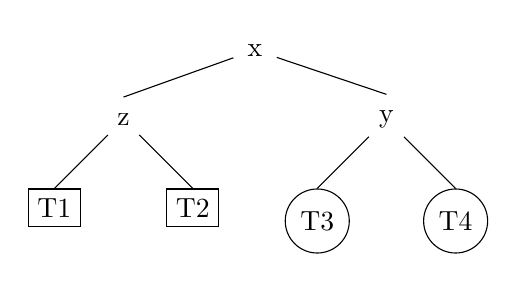
\begin{tikzpicture}[
				level distance = 2.5em,
				level 1/.style={sibling distance=9.5em},
				level 2/.style={sibling distance=5.0em},
				child anchor =north
				]
				\node[circle] (t1) {x}
				child { node[circle]   {z}
					child { node[draw=black, anchor = north]   {T1}
					}
					child { node[draw=black, anchor = north]   {T2}
					}
			}
				child { node[circle]   {y}
					child { node[circle, anchor = north, draw=black] {T3}}
					child { node[circle, anchor = north, draw=black] {T4}
					}
				};
			\end{tikzpicture}
		\column{0.455\textwidth}
		\begin{itemize}
			\item We can now rotate some stuff around :)
			\item Notice that the subtrees have not changed.
				\begin{itemize}
					\item $T1,T3,T4$ have a height of $h$
					\item $T2$ has a height of $h-1$
						
					\item $z$ now has a height of $h+1$
					\item $y$ now has a height of $h+1$
					\item $x$ now has a height of $h+2$
				\end{itemize}
		\end{itemize}
			
	\end{columns}

	
\end{frame}

%%%%%%%%%%%%%%%%%%%%%%%%%%%%%%%%%%%%%%%%%%%%%%%%%%%%%%%%%%%%%%%%%%%%%%
\begin{frame}
	\frametitle{Let's help ourselves}
	\begin{columns}[T]
		\column{0.455\textwidth}
			
			\begin{tikzpicture}[
				level distance = 2.5em,
				level 1/.style={sibling distance=9em},
				level 2/.style={sibling distance=4.5em},
				level 3/.style={sibling distance=3em},
				level 4/.style={sibling distance=2em},
				]
				\node[circle] (t1) {12}
				child { node[circle]   {3}
					child { node[circle] {$\square$} }
					child { node[circle] {9}
						child { node[circle] {$\square$} }
						child { node[circle] {$\square$} }
					}
				}
				child { node[circle]   {25}
					child { node[circle] {14}
						child { node[circle] {$\square$} }
						child { node[circle] {$\square$} }
					}
					child { node[circle] {29}
						child { node[circle] {26}
							child { node[circle] {$\square$} }
							child { node[circle] {27}}
						}
						child { node[circle] {32}
							child { node[circle] {$\square$} }
							child { node[circle] {$\square$} }
						}
					}
				};
			\end{tikzpicture}
		\column{0.455\textwidth}
		\begin{itemize}
			\item Let's draw the non-existing leafs!
			\item This will help us identify what to rotate :)
				
			\item And let's do this on the board.
		\end{itemize}
	\end{columns}
\end{frame}

%%%%%%%%%%%%%%%%%%%%%%%%%%%%%%%%%%%%%%%%%%%%%%%%%%%%%%%%%%%%%%%%%%%%%%
\begin{frame}
	\frametitle{Binary Search Trees}
	\begin{center}
		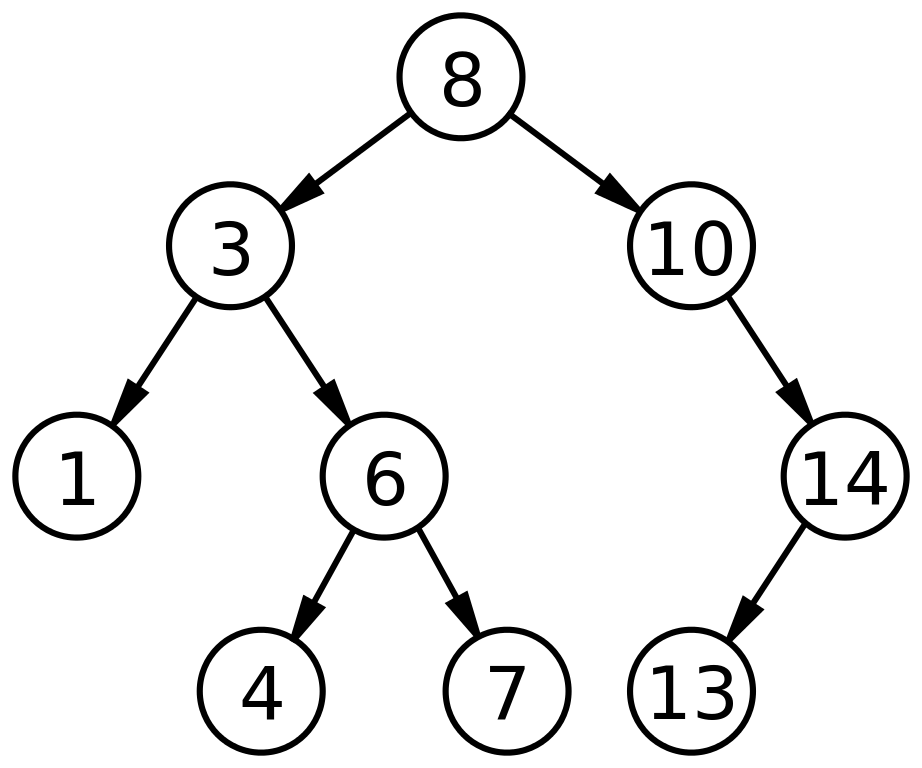
\includegraphics[width=0.5\textwidth]{images/btree.png}\\
		\hspace*{15pt}\hbox{\scriptsize Image By:\thinspace{\itshape Derrick Coetzee}}
		% https://en.wikipedia.org/wiki/File:Binary_search_tree.svg
	\end{center}
\end{frame}

%%%%%%%%%%%%%%%%%%%%%%%%%%%%%%%%%%%%%%%%%%%%%%%%%%%%%%%%%%%%%%%%%%%%%%
\begin{frame}
	\frametitle{Binary Search Trees}
	
		\begin{itemize}
			\item Every node has at most 2 children.
				
			\item The left descendants have a smaller value than the node.
			\item The right descendants have a larger value than the node.
		\end{itemize}
	
	\begin{columns}[T]
		\column{0.455\textwidth}

		\begin{tikzpicture}[
			level distance = 2.5em,
			level 1/.style={sibling distance=9em},
			level 2/.style={sibling distance=4.5em},
			level 3/.style={sibling distance=2.25em},
			]
			\node[circle] (t1) {12}
			child { node[circle]   {3}
				child { node[circle] {2}}
				child { node[circle] {9}}
			}
			child { node[circle]   {25}
				child { node[circle] {14}}
				child { node[circle] {29}
					child { node[circle] {26}}
					child { node[circle] {32}}
				}
			};
		\end{tikzpicture}
		\column{0.455\textwidth}

			Is this tree a binary search tree?
		
			Yes :)	
	\end{columns}
\end{frame}

%%%%%%%%%%%%%%%%%%%%%%%%%%%%%%%%%%%%%%%%%%%%%%%%%%%%%%%%%%%%%%%%%%%%%%
\begin{frame}
	\frametitle{Searching in a Binary SearchTree}
	
			So, how quickly can we search for an item in a Binary Search Tree?
			\begin{itemize}
				\item $\Theta(\log h)$
				\item $\Theta(h)$
				\item $\Theta(\log n)$
				\item $\Theta(n)$
				\item $\Theta($\textit{I don't know man}$)$
			\end{itemize}
		
		Only one path:	So $\Theta(h)$

		\lstinputlisting{src/search_btree.py}
		

\end{frame}

%%%%%%%%%%%%%%%%%%%%%%%%%%%%%%%%%%%%%%%%%%%%%%%%%%%%%%%%%%%%%%%%%%%%%%
\begin{frame}
	\frametitle{MinMaxing}
	
Minmaxing like a real gamer:	So, how quickly can we find the minimum or maximum in a Binary Search Tree?
			\begin{itemize}
				\item $\Theta(\log h)$
				\item $\Theta(h)$
				\item $\Theta(\log n)$
				\item $\Theta(n)$
				\item $\Theta($\textit{Something?}$)$
			\end{itemize}

		Only one path:	So $\Theta(h)$

		\lstinputlisting{src/minmax_btree.py}
	
\end{frame}

%%%%%%%%%%%%%%%%%%%%%%%%%%%%%%%%%%%%%%%%%%%%%%%%%%%%%%%%%%%%%%%%%%%%%%
\begin{frame}
	\frametitle{Inserting or Deleting an item}

			\begin{itemize}
				\item Inserting an item:	Find the right place in $\Theta(h)$ time, then put it there.
				\item Deleting an item:	Find the item in $\Theta(h)$ time, then move either the left or right child up one level (and continue this down the
		path to a leaf).
				\item Sorting the list:		Oh and by the way, this is where the in-order traversal can get us a sorted list of all items in the tree!
		\end{itemize}	
\end{frame}

%%%%%%%%%%%%%%%%%%%%%%%%%%%%%%%%%%%%%%%%%%%%%%%%%%%%%%%%%%%%%%%%%%%%%%
\begin{frame}
	\frametitle{So in summary}
	\begin{tabular}{r | l}
		Operation & Time \\
		\midrule
		Insert & $\Theta(h)$ \\
		Delete & $\Theta(h)$ \\
		Search & $\Theta(h)$ \\
		Min & $\Theta(h)$ \\
		Max & $\Theta(h)$ \\
	\end{tabular}
		
		What is the worst-case $h$, and how do we get that?
	
			\begin{itemize}
				\item Insert a sorted list, and what happens? \\
		 				\item We get a tree with only right children (or only left if the list is sorted descendingly).
	\end{itemize}
	
\end{frame}

%%%%%%%%%%%%%%%%%%%%%%%%%%%%%%%%%%%%%%%%%%%%%%%%%%%%%%%%%%%%%%%%%%%%%%
\begin{frame}
	\frametitle{Generalising a bit}
 search tree:
			\begin{itemize}
				\item Each node of $T$ has \textit{at least} 2 children (except for leaves of course).
				\item Each $d$-node (where $d$ is the amount of children the node has), stores $d-1$ values in increasing value.
				\item Between two keys $i$ and $i+1$ stored in the node, is rooted a tree that contains only keys $k$ such that
					$k_i \leq k \leq k_{i+1}$.
			\end{itemize}
			

		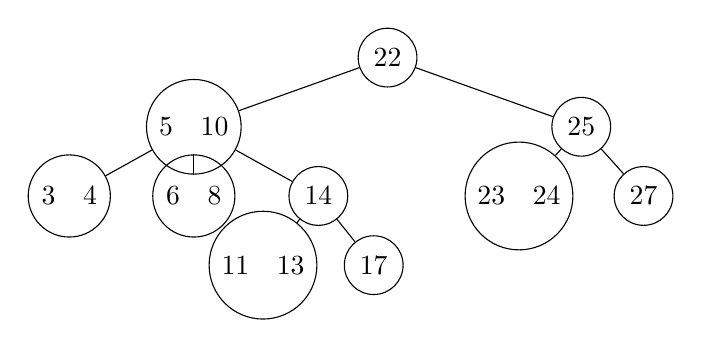
\begin{tikzpicture}[
			level distance = 2.5em,
			level 1/.style={sibling distance=14em},
			level 2/.style={sibling distance=4.5em},
			level 3/.style={sibling distance=2.25em},
			level 3/.style={sibling distance=4em},
			]
			\node[circle, draw] (t1) {22}
			child { node[circle, draw]   {5\quad10}
				child { node[circle, draw] {3\quad4}}
				child { node[circle, draw] {6\quad8}}
				child { node[circle, draw] {14}
					child { node[circle, draw] {11\quad13}}
					child { node[circle, draw] {17}}
				}
			}
			child { node[circle, draw]   {25}
				child { node[circle, draw] {23\quad24}}
				child { node[circle, draw] {27}}
			};
		\end{tikzpicture}
	
\end{frame}

%%%%%%%%%%%%%%%%%%%%%%%%%%%%%%%%%%%%%%%%%%%%%%%%%%%%%%%%%%%%%%%%%%%%%%
\begin{frame}
	\frametitle{Practice?}
	
			\begin{itemize}
				\item You should be able to search for items in a multiway search tree.
				\item And in the lab you will practice a bit with inserting nodes. Read the book carefully, it's not trivial!
				\item On the computer exam, we will not ask you to implement insertion or deletion in multiway search trees.
			\end{itemize}
\end{frame}

%%%%%%%%%%%%%%%%%%%%%%%%%%%%%%%%%%%%%%%%%%%%%%%%%%%%%%%%%%%%%%%%%%%%%%
\begin{frame}
	\frametitle{Recap}
	
Binary Trees:
			\begin{itemize}
				\item Every node has at most 2 children.
					
				\item One \textit{left} child and one \textit{right} child.
			\end{itemize}
		
		A binary tree is \textit{proper} or \textit{full} if all nodes have either 0 or 2 children.
		
		\begin{columns}[T]
			\column{0.455\textwidth}
				
			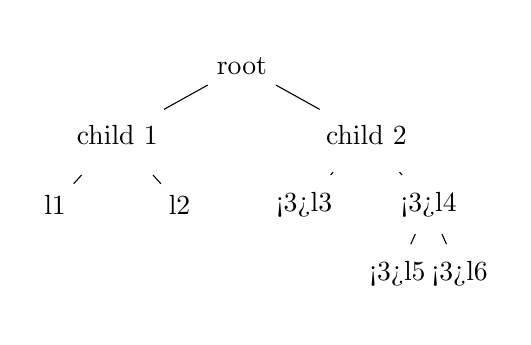
\begin{tikzpicture}[
				level distance = 2.5em,
				level 1/.style={sibling distance=9em},
				level 2/.style={sibling distance=4.5em},
				level 3/.style={sibling distance=2.25em},
			]
			\node[circle] (t1) {root}
				child { node[circle]   {child 1}
					child { node[circle] {l1}}
					child { node[circle] {l2}}
				}
				child { node[circle]   {child 2}
					child { node[circle] {\alert<3>{l3}}}
					child { node[circle] {\alert<3>{l4}}
						child { node[circle] {\alert<3>{l5}}}
						child { node[circle] {\alert<3>{l6}}}
					}
				};
			\end{tikzpicture}
			\column{0.455\textwidth}
				
				Is this tree full?
				
				Yes :)	
		\end{columns}
\end{frame}

%%%%%%%%%%%%%%%%%%%%%%%%%%%%%%%%%%%%%%%%%%%%%%%%%%%%%%%%%%%%%%%%%%%%%%
\begin{frame}
	\frametitle{Recap of Trees}
	\begin{columns}[T]
		\column{0.405\textwidth}
			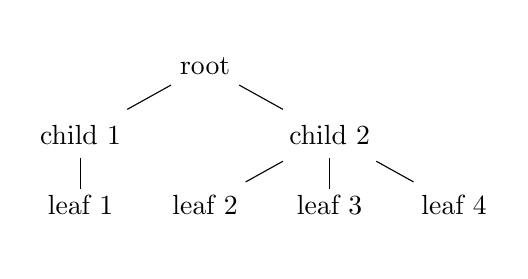
\begin{tikzpicture}[
				level distance = 2.5em,
				level 1/.style={sibling distance=9em},
				level 2/.style={sibling distance=4.5em},
				level 3/.style={sibling distance=2.25em},
			]
			\node[circle] (t1) {root}
				child { node[circle] {child 1}
					child { node[circle] {leaf 1}}
				}
				child { node[circle] {child 2}
					child { node[circle] {leaf 2}}
					child { node[circle] {leaf 3}}
					child { node[circle] {leaf 4}}
				};
			\end{tikzpicture}
		\column{0.555\textwidth}
		\begin{itemize}
			\item The \textit{root node} is the node that has no \textit{parent}.
			\item A node can have \textit{children}.
			\item A node without children is called a \textit{leaf}.
			\item Two nodes with the same \textit{parent} are \textit{siblings}.
			\item \textit{Descendants} are found by repeatedly following child-relations.
			\item \textit{Ancestors} are found by repeatedly following parent-relations.
		\end{itemize}
	\end{columns}
\end{frame}

%%%%%%%%%%%%%%%%%%%%%%%%%%%%%%%%%%%%%%%%%%%%%%%%%%%%%%%%%%%%%%%%%%%%%%
\begin{frame}[fragile]\frametitle{}
\begin{center}
{\Large Heaps}
\end{center}

\end{frame}

%%%%%%%%%%%%%%%%%%%%%%%%%%%%%%%%%%%%%%%%%%%%%%%%%%%%%%%%%%%%%%%%%%%%%%
\begin{frame}
	\frametitle{Heaps}
			We impose extra constraints and create a \textit{heap}:
			\begin{itemize}
				\item \textbf{Heap-order property:} For all nodes: The item stored in a node is greater than the item stored in its parent.
				\item \textbf{Complete Binary Tree property:} The tree is \textit{complete}: Meaning all layers are full, except possibly the last one which has only
					nodes in the left-most positions. 
			\end{itemize}
			
			In this way, it is called a \textit{min-heap}. A \textit{max-heap} has the largest key in the root.
		
		\begin{columns}
			\column{0.455\textwidth}

			\begin{tikzpicture}[
				level distance = 2.5em,
				level 1/.style={sibling distance=9em},
				level 2/.style={sibling distance=4.5em},
				level 3/.style={sibling distance=2.25em},
				]
				\node[circle] (t1) {1}
				child { node[circle]   {12}
					child { node[circle] {14}}
				}
				child { node[circle]   {4}
					child { node[circle] {5}}
					child { node[circle] {17}}
				};
			\end{tikzpicture}
			\column{0.455\textwidth}

				Is this a correct min-heap?
			
				No, as we do not use the left-most spots in the bottom layer.
		\end{columns}
\end{frame}

%%%%%%%%%%%%%%%%%%%%%%%%%%%%%%%%%%%%%%%%%%%%%%%%%%%%%%%%%%%%%%%%%%%%%%
\begin{frame}
	\frametitle{A use case}
	\begin{columns}
		\column{0.455\textwidth}
	\begin{center}

					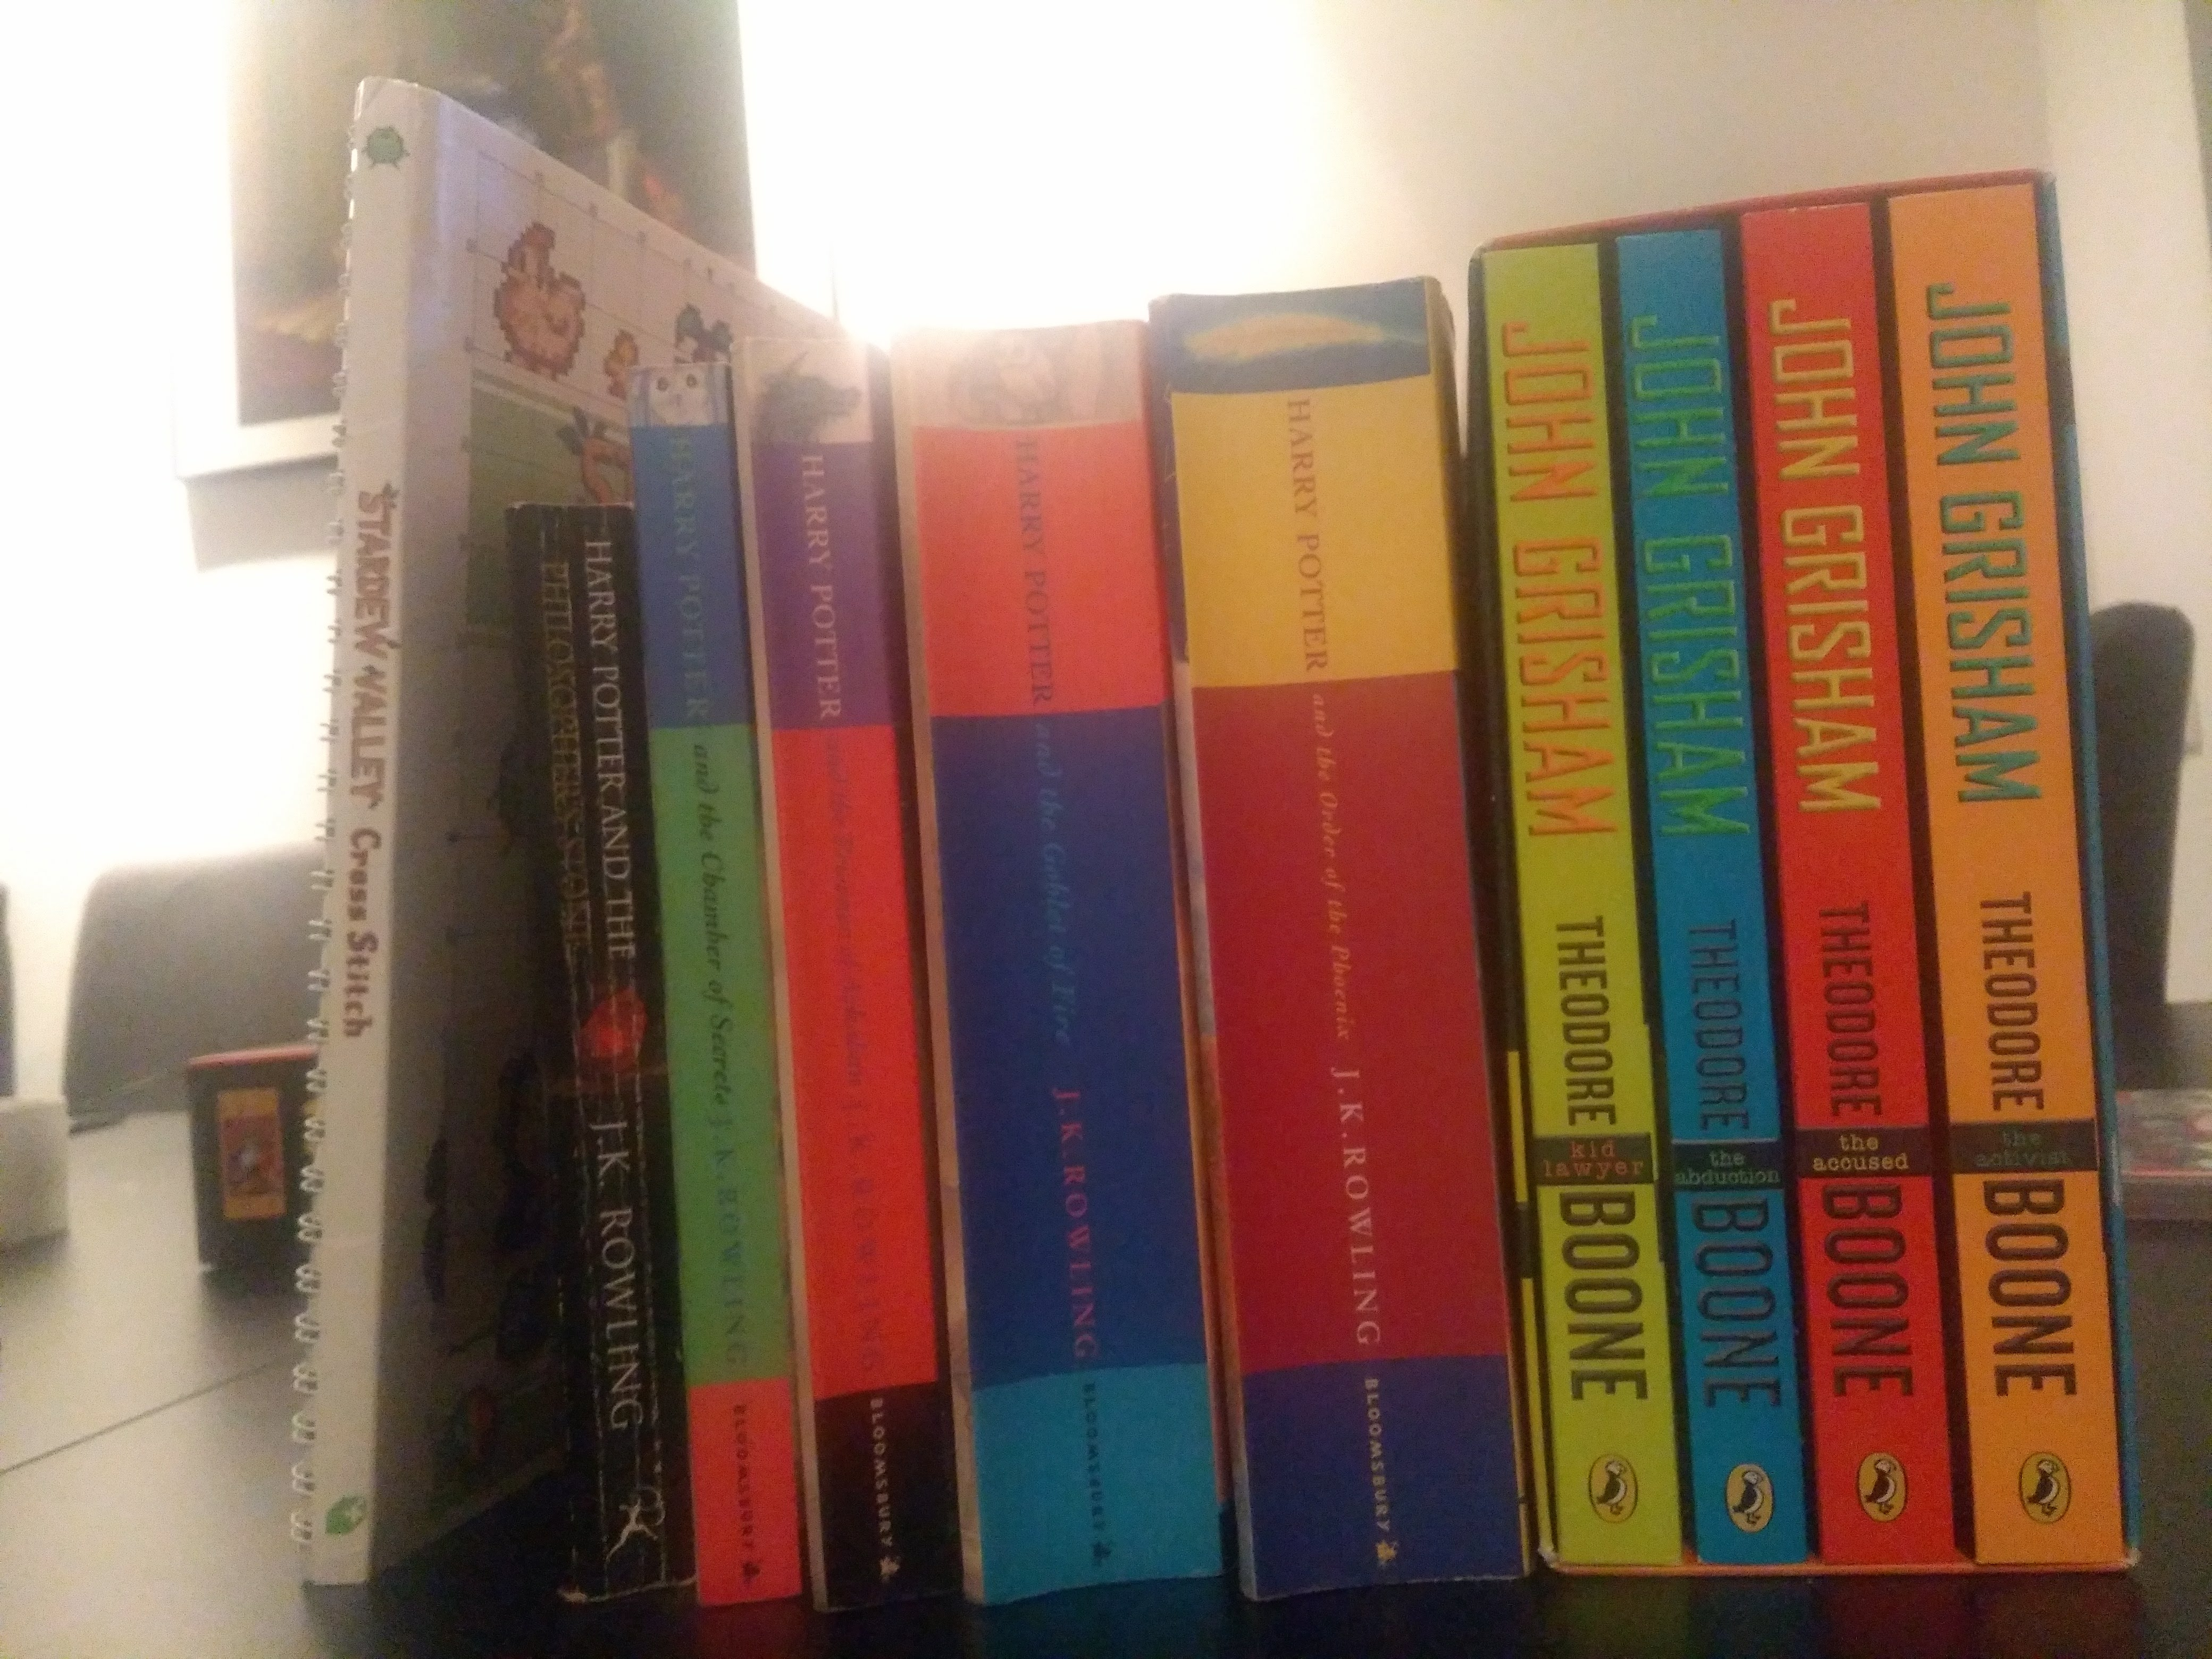
\includegraphics[width=0.5\textwidth]{images/books_read.jpg}
	
					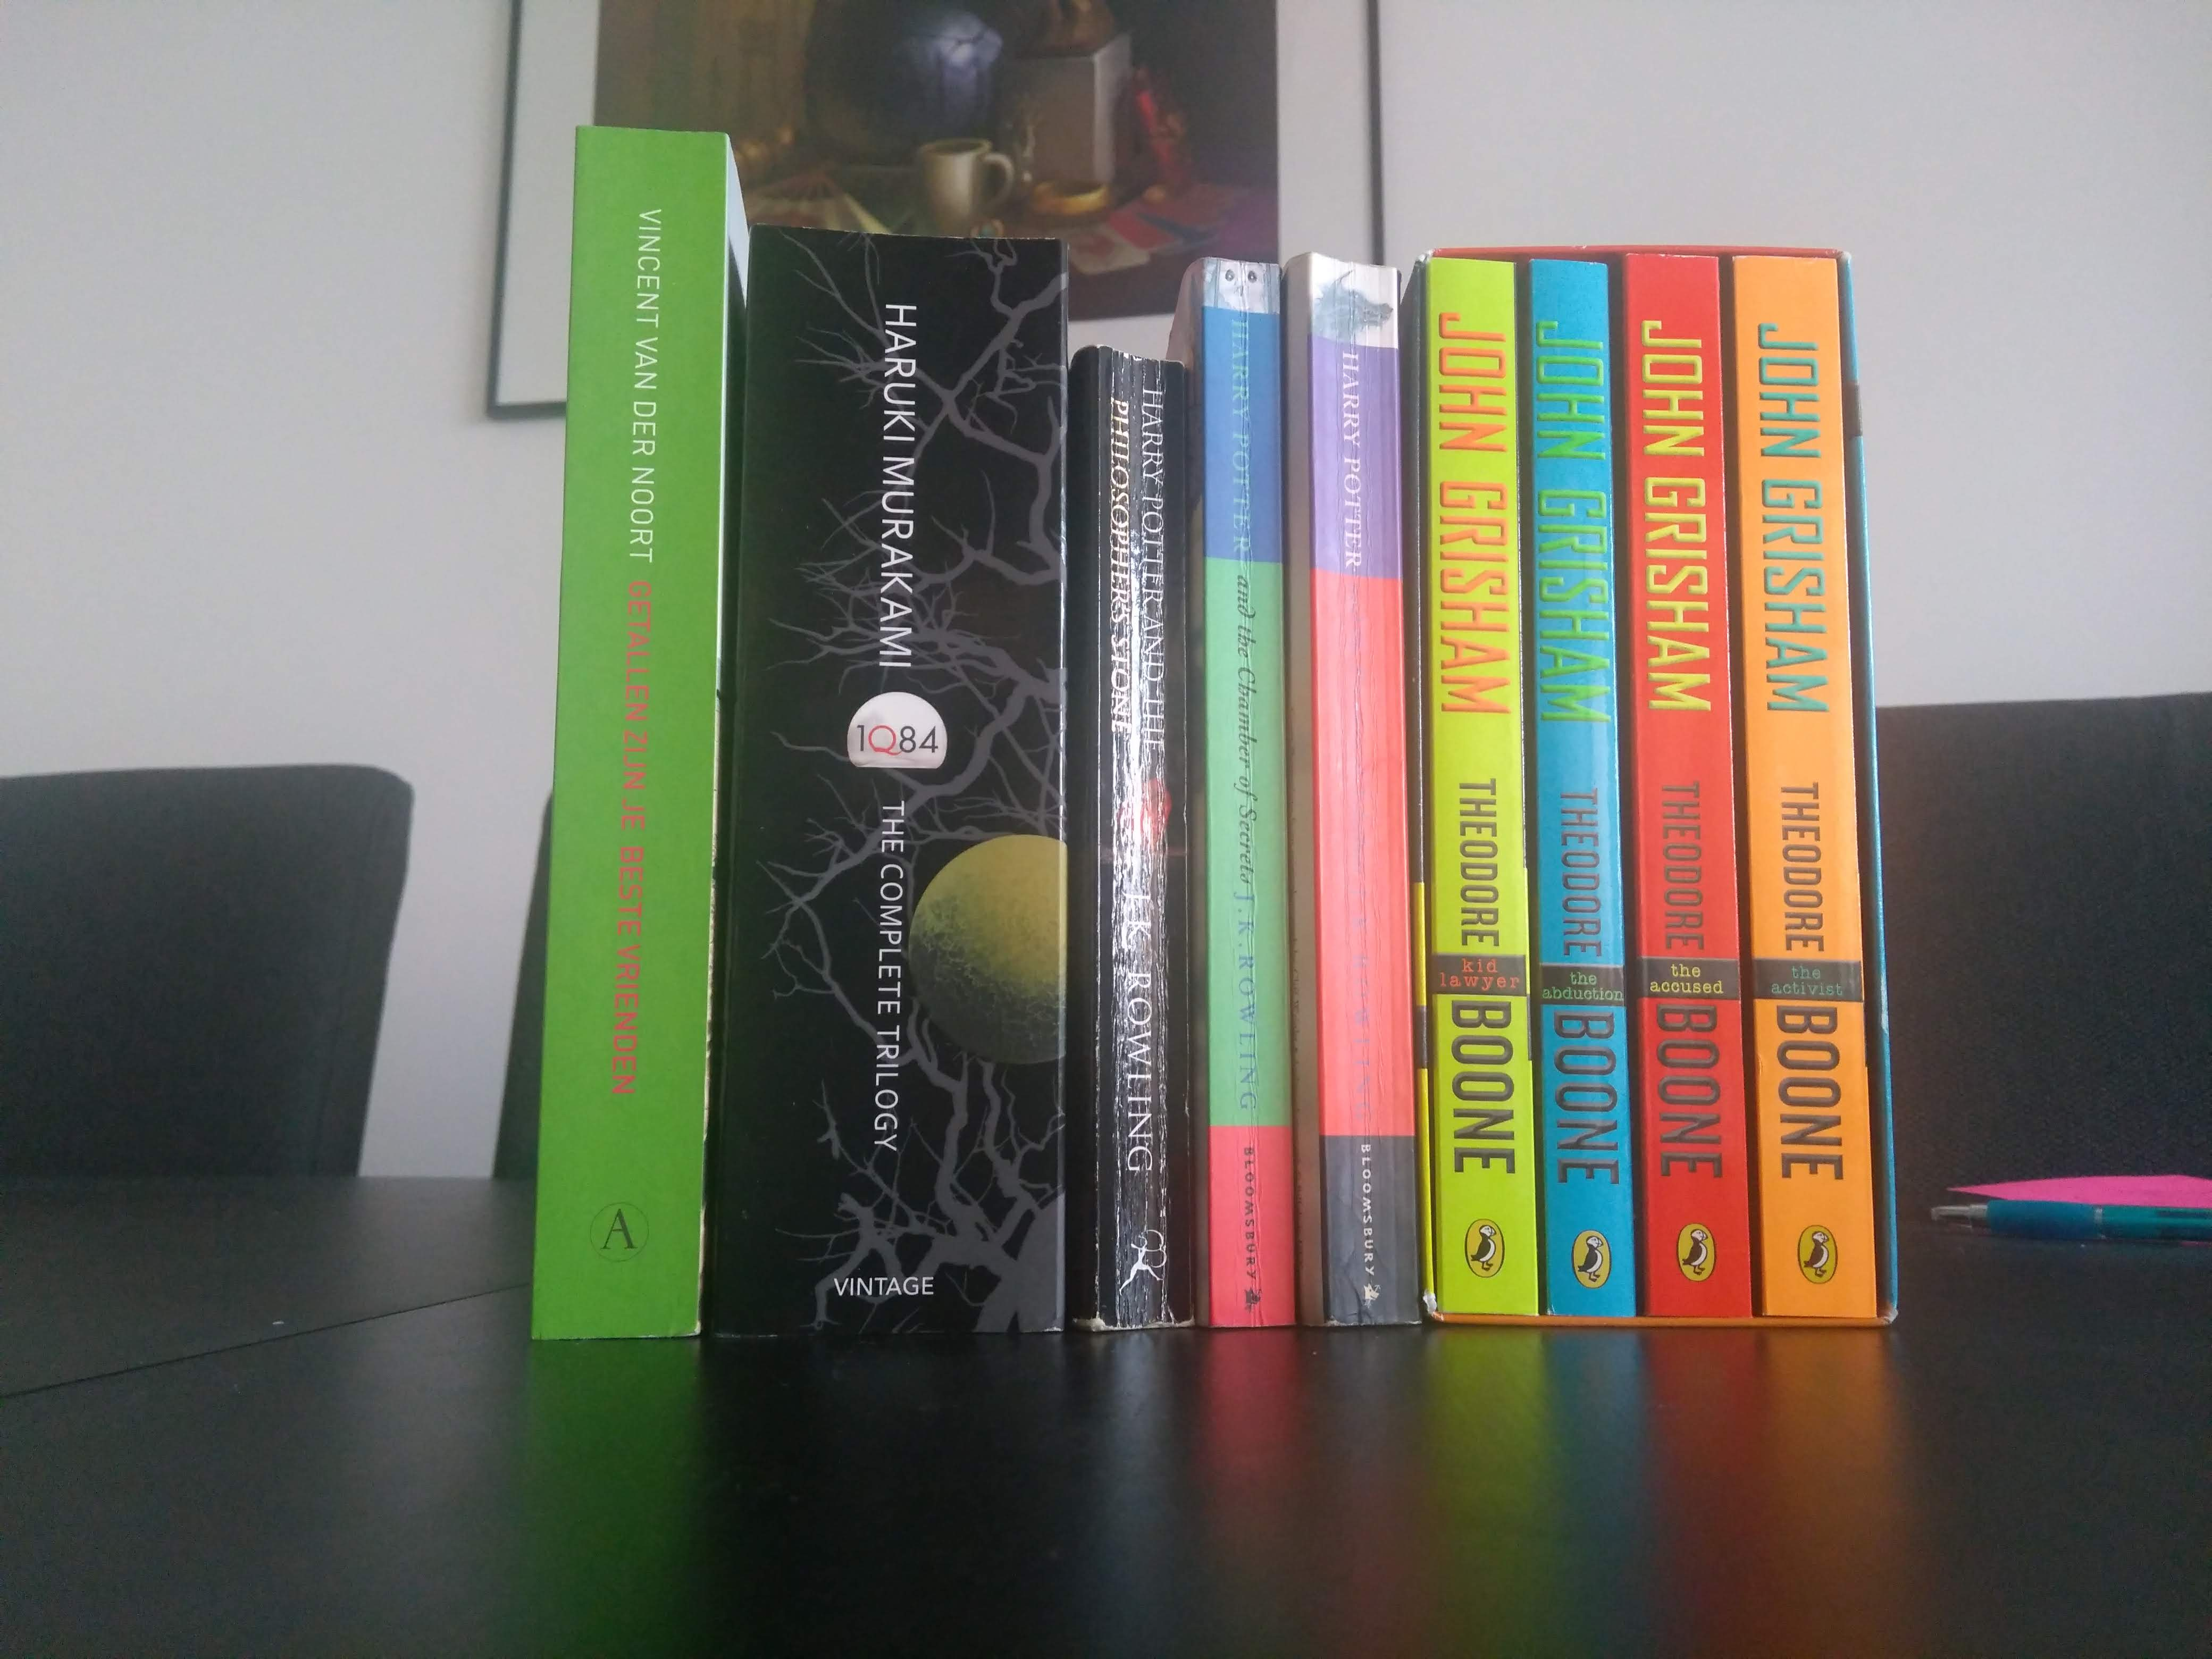
\includegraphics[width=0.5\textwidth]{images/books_unread.jpg}

{\scriptsize Image By:\thinspace{\itshape Stefan Hugtenburg}}
{\scriptsize Bookcovers and picture in the back by others}
	\end{center}
		\column{0.455\textwidth}
		\begin{itemize}
			\item There is more room for improvement.
				
			\item A nice \alert{queue} of books.
				
			\item After finishing one, I would take the next one from the left.
				
			\item But what if a book should get \textit{priority}?
				
			\item This uses a \textit{Priority Queue}, which we discuss in detail today.
		\end{itemize}
	\end{columns}
\end{frame}



%%%%%%%%%%%%%%%%%%%%%%%%%%%%%%%%%%%%%%%%%%%%%%%%%%%%%%%%%%%%%%%%%%%%%%
\begin{frame}
	\frametitle{A PriorityQueue ADT: A Heap ADT}
Heap, Heap, Array: There is no heap ADT per sé, it's just a special type of tree.
		
PriorityQueue: 	But there is one for a PriorityQueue (which we could implement using a heap):
			\begin{itemize}
				\item \texttt{size()} (or \texttt{len} in Python) to get the number of elements.
					
				\item \texttt{add(item)} to insert an item into the queue.
					
				\item \texttt{remove\_min()} to remove the smallest element from the queue.
					
				\item \texttt{min()} to get the smallest element from the queue.
			\end{itemize}
\end{frame}

%%%%%%%%%%%%%%%%%%%%%%%%%%%%%%%%%%%%%%%%%%%%%%%%%%%%%%%%%%%%%%%%%%%%%%
\begin{frame}
	\frametitle{An array-based Priority Queue}


	\begin{columns}[T]
		\column{0.455\textwidth}
		\lstinputlisting{src/pq_array.py}
		\column{0.455\textwidth}
		
			\begin{itemize}
				\item Array-based PQ:	We can easily create a PQ based on an array (or list).
				\item But this makes \texttt{min} and \texttt{remove\_min} linear time operations!
				\item Can we do better by using a sorted array?
							\end{itemize}

	\end{columns}
\end{frame}

%%%%%%%%%%%%%%%%%%%%%%%%%%%%%%%%%%%%%%%%%%%%%%%%%%%%%%%%%%%%%%%%%%%%%%
\begin{frame}
	\frametitle{An sorted array-based Priority Queue}

	\begin{columns}[T]
		\column{0.455\textwidth}
		\lstinputlisting{src/pq_sortedarray.py}
		\column{0.455\textwidth}
		
			\begin{itemize}
				\item Array-based PQ:	We can easily create a PQ based on a sorted array (or list).
				\item But this makes \texttt{remove\_min} and \texttt{add} linear time operations!
				\item Can we do better by using a heap?
			\end{itemize}
	\end{columns}
\end{frame}

%%%%%%%%%%%%%%%%%%%%%%%%%%%%%%%%%%%%%%%%%%%%%%%%%%%%%%%%%%%%%%%%%%%%%%
\begin{frame}
	\frametitle{Min in a heap}
		How do I implement \texttt{min} for my heap-based PQ?
		\begin{itemize}
			\item Return the value in the root.
			\item Return the value of the left-most descendant.
			\item Return the value of the right-most descendant.
			\item Go over all elements and return the minimum.
		\end{itemize}

\end{frame}

%%%%%%%%%%%%%%%%%%%%%%%%%%%%%%%%%%%%%%%%%%%%%%%%%%%%%%%%%%%%%%%%%%%%%%
\begin{frame}
	\frametitle{Adding in a heap}
		Consider the following heap:
		\begin{columns}[T]
			\column{0.455\textwidth}
			\begin{tikzpicture}[
				level distance = 2.5em,
				level 1/.style={sibling distance=9em},
				level 2/.style={sibling distance=4.5em},
				level 3/.style={sibling distance=2.25em},
				]
				\node[circle] (t1) {1}
				child { node[circle]   {12}
					child { node[circle] {14}}
					child { node[circle] {17}}
				}
				child { node[circle]   {4}
					child { node[circle] {5}}
				};
			\end{tikzpicture}
			\column{0.455\textwidth}
			
			If I insert the element $7$ here, what should I do?
		\end{columns}
Just add it at the bottom-right!
			\begin{tikzpicture}[
				level distance = 2.5em,
				level 1/.style={sibling distance=9em},
				level 2/.style={sibling distance=4.5em},
				level 3/.style={sibling distance=2.25em},
				scale=0.8, transform shape
				]
				\node[circle] (t1) {1}
				child { node[circle]   {12}
					child { node[circle] {14}}
					child { node[circle] {17}}
				}
				child { node[circle]   {4}
					child { node[circle] {5}}
					child { node[circle] {7}}
				};
			\end{tikzpicture}
\end{frame}

%%%%%%%%%%%%%%%%%%%%%%%%%%%%%%%%%%%%%%%%%%%%%%%%%%%%%%%%%%%%%%%%%%%%%%
\begin{frame}
	\frametitle{Adding in a heap}
		Consider the following heap:
		\begin{columns}[T]
			\column{0.455\textwidth}
			\begin{tikzpicture}[
				level distance = 2.5em,
				level 1/.style={sibling distance=9em},
				level 2/.style={sibling distance=4.5em},
				level 3/.style={sibling distance=2.25em},
				]
				\node[circle] (t1) {1}
				child { node[circle]   {12}
					child { node[circle] {14}}
					child { node[circle] {17}}
				}
				child { node[circle]   {4}
					child { node[circle] {5}}
				};
			\end{tikzpicture}
			\column{0.455\textwidth}
			
			If I insert the element $0$ here, what should I do?
		\end{columns}
Just add it at the bottom-right!
		\begin{columns}[T]
			\column{0.455\textwidth}
			\begin{tikzpicture}[
				level distance = 2.5em,
				level 1/.style={sibling distance=9em},
				level 2/.style={sibling distance=4.5em},
				level 3/.style={sibling distance=2.25em},
				scale=0.8, transform shape
				]
				\node[circle] (t1) {1}
				child { node[circle]   {12}
					child { node[circle] {14}}
					child { node[circle] {17}}
				}
				child { node[circle]   {4}
					child { node[circle] {5}}
					child { node[circle] {0}}
				};
			\end{tikzpicture}
			\column{0.455\textwidth}
			
			And now fix the damage we have caused :)
		\end{columns}
\end{frame}

%%%%%%%%%%%%%%%%%%%%%%%%%%%%%%%%%%%%%%%%%%%%%%%%%%%%%%%%%%%%%%%%%%%%%%
\begin{frame}
	\frametitle{Up-bubbling}

Fixing the damage:	How can we fix the damage caused to the heap \textit{efficiently}?
		\begin{columns}[T]
			\column{0.455\textwidth}
			\begin{tikzpicture}[
				level distance = 2.5em,
				level 1/.style={sibling distance=9em},
				level 2/.style={sibling distance=4.5em},
				level 3/.style={sibling distance=2.25em},
				scale=0.8, transform shape
				]
				\node[circle] (t1) {1}
				child { node[circle]   {12}
					child { node[circle] {14}}
					child { node[circle] {17}}
				}
				child { node[circle]   {4}
					child { node[circle] {5}}
					child { node[circle] {0}}
				};
			\end{tikzpicture}
			\column{0.455\textwidth}
			
			\begin{itemize}
				\item Swap it with the root element and then swap it down as needed.
				\item Repeatedly compare the new node with the siblings and swap if needed.
				\item Repeatedly compare the new node with the parent and swap if needed.
				\item We cannot, we have to rebuild the entire heap.
			\end{itemize}
		\end{columns}
\end{frame}

% %%%%%%%%%%%%%%%%%%%%%%%%%%%%%%%%%%%%%%%%%%%%%%%%%%%%%%%%%%%%%%%%%%%%%%
% \begin{frame}
	% \frametitle{Up-bubbling}

% Fixing the damage:		Repeatedly switch with the parent if needed.
		% \begin{columns}[T]
			% \column{0.455\textwidth}
				
			% \begin{tikzpicture}[
				% level distance = 2.5em,
				% level 1/.style={sibling distance=9em},
				% level 2/.style={sibling distance=4.5em},
				% level 3/.style={sibling distance=2.25em},
				% scale=0.8, transform shape
				% ]
				% \node[circle] (t1) {1}
				% child { node[circle]   {12}
					% child { node[circle] {14}}
					% child { node[circle] {17}}
				% }
				% child { node[circle] {1}{4}
					% child { node[circle] {5}}
					% child { node[circle] {4}{0}}
				% }
			% \end{tikzpicture}
			% \column{0.455\textwidth}

			% \begin{itemize}
				% \item Notice how the left half of the tree has not been touched at all!
				% \item Only one path changes!
			% \end{itemize}	

		% \end{columns}
% \end{frame}

% %%%%%%%%%%%%%%%%%%%%%%%%%%%%%%%%%%%%%%%%%%%%%%%%%%%%%%%%%%%%%%%%%%%%%%
% \begin{frame}
	% \frametitle{Up-bubbling pt2}
			% \begin{tikzpicture}[
				% level distance = 2.5em,
				% level 1/.style={sibling distance=9em},
				% level 2/.style={sibling distance=4.5em},
				% level 3/.style={sibling distance=2.25em},
				% scale=0.8, transform shape
				% ]
				% \node[circle] (t1) {6}
				% child { node[circle]   {14}
					% child { node[circle] {17}}
					% child { node[circle] {21}}
				% }
				% child { node[circle]   {8}
					% child { node[circle] {18}}
					% child { node[circle] {9}}
				% };
			% \end{tikzpicture}
% Where does it go?:
				% Try to insert the element $10$ in this heap. Where does it end up?
				% \begin{itemize}
					% \item As the root
					% \item At depth 1
					% \item At depth 2
					% \item At depth 3
				% \end{itemize}
% \end{frame}

% %%%%%%%%%%%%%%%%%%%%%%%%%%%%%%%%%%%%%%%%%%%%%%%%%%%%%%%%%%%%%%%%%%%%%%
% \begin{frame}
	% \frametitle{Removing from a heap}
		% Consider the following heap:
		% \begin{columns}[T]
			% \column{0.455\textwidth}
			% \begin{tikzpicture}[
				% level distance = 2.5em,
				% level 1/.style={sibling distance=9em},
				% level 2/.style={sibling distance=4.5em},
				% level 3/.style={sibling distance=2.25em},
				% ]
				% \node[circle] (t1) {1}
				% child { node[circle]   {12}
					% child { node[circle] {14}}
					% child { node[circle] {17}}
				% }
				% child { node[circle]   {4}
					% child { node[circle] {5}}
					% child { node[circle] {7}}
				% };
			% \end{tikzpicture}
			% \column{0.455\textwidth}
			
			% If I want to remove the minimum, what should I do?
		% \end{columns}
% Just remove it at the top!
		% \begin{columns}[T]
			% \column{0.455\textwidth}
			% \begin{tikzpicture}[
				% level distance = 2.5em,
				% level 1/.style={sibling distance=9em},
				% level 2/.style={sibling distance=4.5em},
				% level 3/.style={sibling distance=2.25em},
				% scale=0.8, transform shape
				% ]
				% \node[circle] (t1) {$\square$}
				% child { node[circle]   {12}
					% child { node[circle] {14}}
					% child { node[circle] {17}}
				% }
				% child { node[circle]   {4}
					% child { node[circle] {5}}
					% child { node[circle] {7}}
				% };
			% \end{tikzpicture}
			% \column{0.455\textwidth}
			
			% And now fix the damage we have caused :)
		% \end{columns}
% \end{frame}

% %%%%%%%%%%%%%%%%%%%%%%%%%%%%%%%%%%%%%%%%%%%%%%%%%%%%%%%%%%%%%%%%%%%%%%
% \begin{frame}
	% \frametitle{Fixing the damage}
% Just remove it at the top!
		% \begin{columns}[T]
			% \column{0.455\textwidth}
			% \begin{tikzpicture}[
				% level distance = 2.5em,
				% level 1/.style={sibling distance=9em},
				% level 2/.style={sibling distance=4.5em},
				% level 3/.style={sibling distance=2.25em},
				% scale=0.8, transform shape
				% ]
				% \node[circle] (t1) {$\square$}
				% child { node[circle]   {12}
					% child { node[circle] {14}}
					% child { node[circle] {17}}
				% }
				% child { node[circle]   {4}
					% child { node[circle] {5}}
					% child { node[circle] {7}}
				% };
			% \end{tikzpicture}
			% \column{0.455\textwidth}
			
			% What should we do?
			% \begin{itemize}[
				% \item Repeatedly move the smallest child up.
				% \item First move the bottom right to the root and then repeatedly swap down with the smallest child.
				% \item Always get the smallest element from the next layer and move it up (so not restricted to your children).
				% \item Nothing, we should just rebuild the heap from scratch.
			% \end{itemize}
		% \end{columns}

% \end{frame}

% %%%%%%%%%%%%%%%%%%%%%%%%%%%%%%%%%%%%%%%%%%%%%%%%%%%%%%%%%%%%%%%%%%%%%%
% \begin{frame}
	% \frametitle{Down-bubbling}

% Fixing the damage: 		First move the bottom-right element to the top, then repeatedly bubble down.
		% \begin{columns}[T]
			% \column{0.455\textwidth}
				
			% \begin{tikzpicture}[
				% level distance = 2.5em,
				% level 1/.style={sibling distance=9em},
				% level 2/.style={sibling distance=4.5em},
				% level 3/.style={sibling distance=2.25em},
				% scale=0.8, transform shape
				% ]
				% \node[circle] (t1) {4}{7}{$\square$}}}}
				% child { node[circle]   {12}
					% child { node[circle] {14}}
					% child { node[circle] {17}}
				% }
				% child { node[circle] {5}{4}}
					% child { node[circle] {7}{5}}}
					% child { node[circle] {$\square$}{7}}}
				% };
			% \end{tikzpicture}
			% \column{0.455\textwidth}
			% \begin{itemize}
				% \item Notice how the left half of the tree has not been touched at all!
				% \item Only one path changes, after the initial switch!
			% \end{itemize}	
	% }
		% \end{columns}
% \end{frame}

%%%%%%%%%%%%%%%%%%%%%%%%%%%%%%%%%%%%%%%%%%%%%%%%%%%%%%%%%%%%%%%%%%%%%%
\begin{frame}
	\frametitle{Down-bubbling pt2}
			\begin{tikzpicture}[
				level distance = 2.5em,
				level 1/.style={sibling distance=9em},
				level 2/.style={sibling distance=4.5em},
				level 3/.style={sibling distance=2.25em},
				scale=0.8, transform shape
				]
				\node[circle] (t1) {6}
				child { node[circle]   {14}
					child { node[circle] {17}
						child { node[circle] {19}}
					}
					child { node[circle] {21}
					}
				}
				child { node[circle]   {8}
					child { node[circle] {18}}
					child { node[circle] {12}
					}
				};
			\end{tikzpicture}
			
				Remove the minimum from the heap, where does $18$ end up?
				
				\begin{itemize}
					\item As the root
					\item At depth 1
					\item At depth 2
					\item At depth 3
				\end{itemize}
\end{frame}
